\documentclass[UTF8]{article}
\usepackage{ctex}
\usepackage{ulem}
\usepackage{dsfont}
\usepackage{amssymb}
\usepackage{amsmath}
\usepackage{graphicx}
\newtheorem{thm}{定义}[section]
\newtheorem{notation}[thm]{记号}
\newtheorem{lemma}[thm]{引理}

\makeatletter
\newcommand{\rmnum}[1]{\romannumeral #1}
\newcommand{\Rmnum}[1]{\expandafter\@slowromancap\romannumeral #1@}
\makeatother
\newcommand{\dperp}{\perp\!\!\!\perp}

\title{13 集合与子集\\Sets and subsets\\[2ex]\begin{large}读书笔记\end{large}}
\author{许博}
\date{}

\begin{document}
\maketitle
	\section{在$\lambda{\rm D}$中处理子集}
	\noindent
	之前我们已经在类型理论中,将类型解释为集合,但当考虑到子集时,会有诸多问题需要考虑。比如类型的唯一性与对子集的自然观点矛盾,假设$S$是一个集合而$T$是$S$的真子集,令$c\in S$,则应有$c\in T$,也即$c:S\Rightarrow c:T$,显然违背了类型唯一性。
		
		另一个例子是,令$P$是$S$中的元素的一个属性,集合$\{x\in S|Px\}$表示$S$中满足$P$的所有元素,则对于$c:S$,$c:\{x\in S|Px\}$是不可判定的,因为在类型理论中,类型检查需要是可判定的,即给定的合法的项,一定能够得它的类型匹配与否,而非尚未知晓的答案,且判定任意命题可证明是不可判定的。
		
		类型的可判定性使得类型理论称为用于证明检查与查找的一个强大系统,另一方面,阻止了对于子集的一般处理方式。而类型理论的可判定性以及类型的唯一性需要得到保留,以使我们的推导系统保持作为证明检查基础的有效性。因此,我们决定保留类型理论的可判定性,以及接受这个选择所带来的所有后果,尤其是关于子集的。
		
		在描述子集的表示方式之前,首先介绍数学中与集合有关的一些概念。
		
		$x\in S$表示$x$是$S$的一个成员。$S$是$T$一个子集,如果$S$的所有成员都是$T$的成员。除此之外还有集合的相等性,并集,交集,差集,补集,幂集以及笛卡尔积等概念,可自行查阅。
		
		在类型理论$\lambda{\rm D}$中,我们通过一种顺理成章又精彩的方式表示子集:使用谓词。假设存在一个集合$S$,集合$V$是$S$中满足谓词$P$的元素的集合,也即$V\subseteq S$,显然对于任意的$x:S$,都有$x\in V\Leftrightarrow P(x)$。此时,我们使用谓词$P$来表示子集$V$,此时对于$S$的子集$V$而言,$V$是在$S$上的谓词。如果$x\in V$,则$Vx$成立。子集的表示如下:\\
		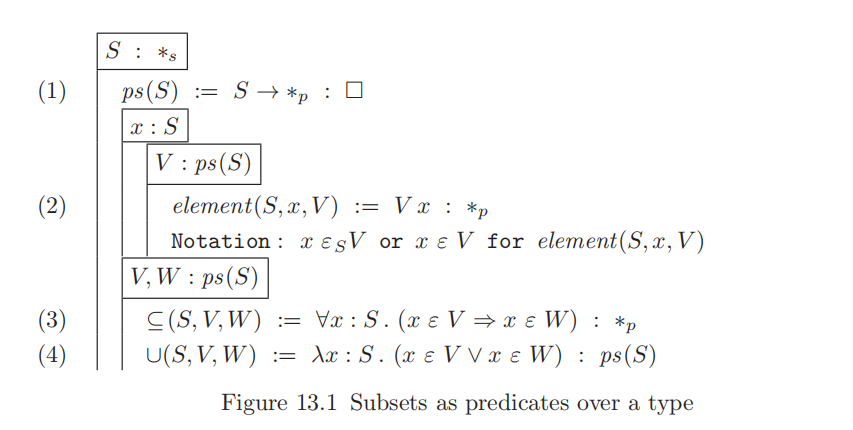
\includegraphics[width=0.93\linewidth]{"../imgs/13-1.png"}
		
		其中,$ps(S)$表示$\mathcal{P}(S)$,也即集合$S$的幂集,可见$ps(S)$的成员均是$S$的子集,也即在$S$上的谓词。同时还定义了关系$\subseteq$和$\cup$。
		
	\section{基础集合论概念}
	\noindent
	本节考虑关于(子)集合的一些概念以及如何在$\lambda{\rm D}$中形式化它们。关键点在于被形式化为谓词的只有子集。概念$x\in V$等价于$x\varepsilon V$而非$x:V$,同时$x\varepsilon V$是一个类型。为了确定$x\varepsilon V$,需要构建一个证明项$p:x\varepsilon V$。
		
		令$S$是一个解释为集合的类型,$V$是$S$的一个子集,$V$是在$S$上的一个谓词,所以我们有$S:*_s$,但是$V:S\rightarrow*_p$。假设我们期望量词作用于子集$V$,如$\forall_{x\in V}(P(x))$,其中$P$是一个谓词,则不能直接形式化为$\forall x:V.Px$,因为$V$不是一个类型。解决方式是量词作用于集合$S$,通过以必须满足谓词$V$的条件以限制定义域,因此使用如下转换:
		
		$\forall_{x\in V}(P(x))\rightsquigarrow \forall x:S.(x\varepsilon V\Rightarrow Px)$
		
		对于存在量词,使用相似的方式:
		
		$\exists_{x\in V}(P(x))\rightsquigarrow \exists x:S.(x\varepsilon V\land Px)$
		
		可以观察到两者之间分别使用了$\Rightarrow$和$\rightsquigarrow$,目的是令不满足子集谓词的成员不影响整个命题的真值。
		
		在图13.2中,使用子集推导式$\{x:S|Vx\}$表示$\lambda x:S.Vx$,将$V x$写作$x\varepsilon V$,可以得到$\{x:S|x\varepsilon V\}$。
		
		以及对于作为类型的集合$S$的子集,和$S$的子集的子集,应用如下变换:\\
		- 若$V$是类型$S$的一个子集,则$V:ps(S)$,或$V:S\rightarrow*_p$\\
		- 若$V$是$S$的一个子集$W$的一个子集,则$V\subseteq W$,或$\forall x:S.(x\varepsilon V\Rightarrow x\varepsilon W)$
		
		在图13.2中,定义了子集间的包括和相等,同时定义了子集间的并集,交集,差集,结果同样是子集,以及关于$S$的补集:\\
		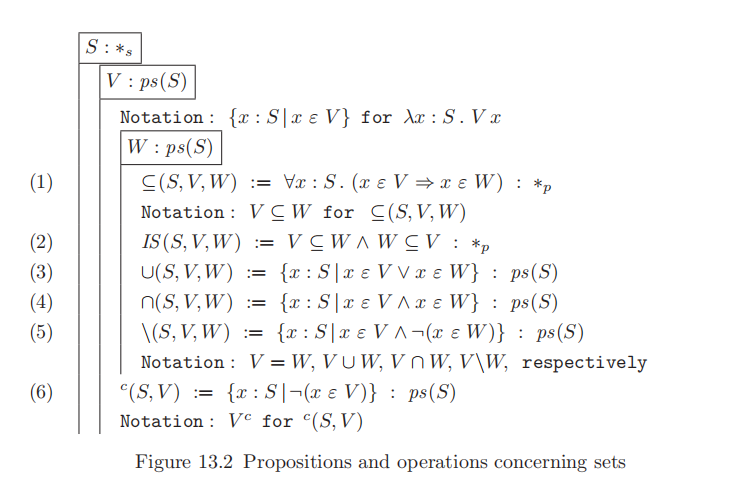
\includegraphics[width=0.93\linewidth]{"../imgs/13-2.png"}
		
		同时非正式地定义了对应操作的中缀形式的语法糖,这些语法糖并未标识出基础的集合$S$,而且,我们重载了符号“=”,因为之前定义的“=”用于元素,现在可以用于子集。
		
		考虑表达式$y\varepsilon\{x:S|Px\}$,等价于$(\lambda x:S.Px)y$,$\beta$-等价于$Py$。$\beta$-等价可以用于$\varepsilon$的引入和消去规则:\\
		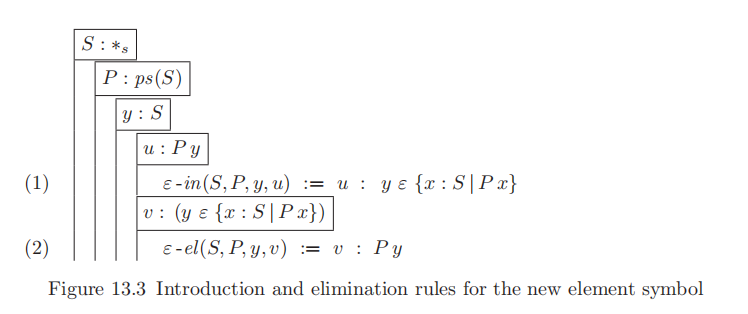
\includegraphics[width=0.93\linewidth]{"../imgs/13-3.png"}
		
		为了展示这些集合的概念如何工作,给出一个简单的类型论定义的证明,证明定理:
		
		\textit{对于$S$的所有子集$V$和$W$,如果$V\subseteq W^c$,则$V\setminus W=V$}。
		
		证明如下:\\
		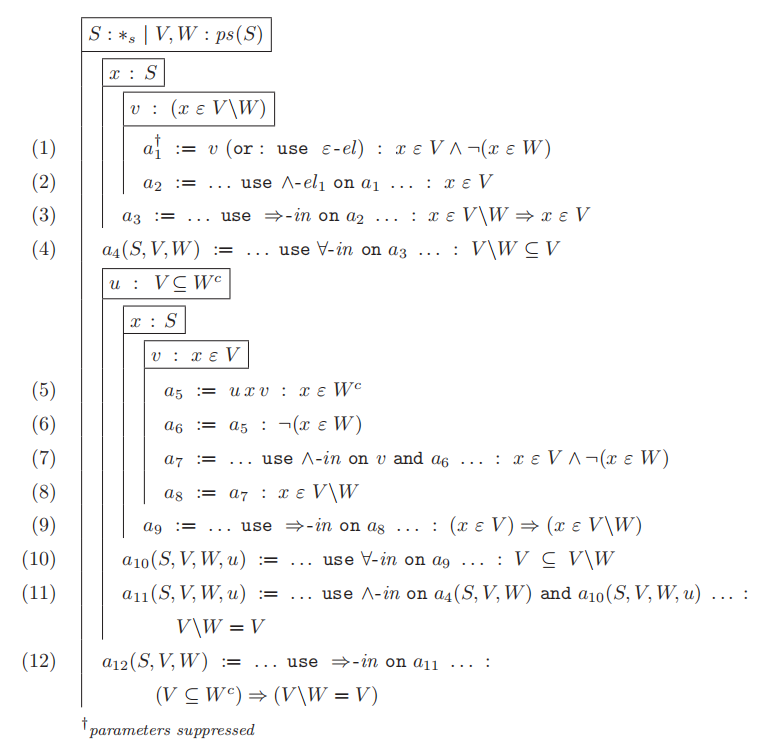
\includegraphics[width=0.93\linewidth]{"../imgs/13-4.png"}
		
		需要注意的是,在证明过程中省略了一些基于逻辑规则的证明项,使用了注解的形式而非正式的使用标准形式的定义实例化,以提高可读性。
		
		本节中所涉及到的概念还剩下一个问题:我们所定义的子集的等价$IS(S,V,W)$,与在章节12.2中讨论的莱布尼兹等价如何联系?
		
		首先我们有$S:*_p$,但是$ps(S):\square$,因此不能使用$V=_{ps(S)}W$以表示$V$和$W$的莱布尼兹等价,但是可以定义相似的在$S$的幂集上的莱布尼兹等价:$\Pi K:ps(S)\rightarrow*_p.(KV\Leftrightarrow KW)$,使用$V\stackrel{\wedge}{=}_{ps(S)}W$表示。
		
		莱布尼兹等价易于证明子集等价,但翻转之后不能构建出我们需要的证明。因此需要添加另一个公理:\\
		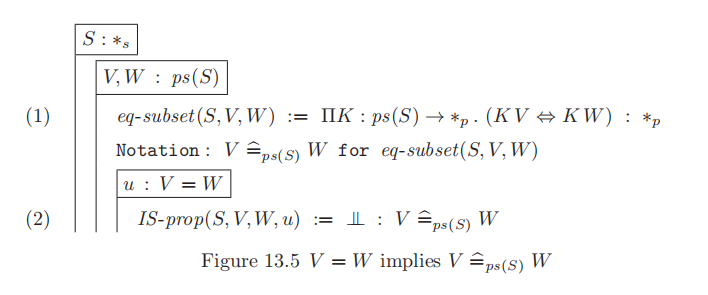
\includegraphics[width=0.93\linewidth]{"../imgs/13-5.png"}
\end{document}
